\documentclass[9pt,aspectratio=169]{beamer}

\usepackage{scalerel}

\usetheme{graham}

\title{Number Theory 101}
\subtitle[Graham Middle School]{Graham Middle School Math Olympiad Team}

\setcounter{MaxMatrixCols}{20}
\newcommand{\Mod}[1]{\ (\mathrm{mod}\ #1)}
\newcommand{\longdiv}{\smash{\mkern-0.43mu\vstretch{1.31}{\hstretch{.7}{)}}\mkern-5.2mu\vstretch{1.31}{\hstretch{.7}{)}}}}

\newcommand\Mydiv[2]{%
$\strut#1$\kern.25em\smash{\raise.3ex\hbox{$\big)$}}$\mkern-8mu
        \overline{\enspace\strut#2}$}

\DeclareMathOperator{\lcm}{lcm}

\begin{document}
\maketitle

\begin{frame}{Number Theory definitions}
  \begin{columns}[T]
    \begin{column}{0.5\textwidth}
      \textbf{Counting Numbers} = $\{1,\ 2,\ 3,\ \ldots\}$ is the numbers we use for counting. 
      
      (Yes, this is the definition.)

      The brackets here mean “the set including.” 
      
      Mathematicians use $\mathbb{N}$ as the symbol for this set.\medskip

      \textbf{Whole Numbers} = $\{0,\ 1,\ 2,\ 3,\ \ldots\}$, so this is the set of counting numbers plus the element zero. 
      
      Mathematicians use $\mathbb{N}_0$ or $\mathbb{Z}_+$ as the symbol for this set.\medskip

      \textbf{Integers} = $\{\ldots,\ –3,\ –2,\ –1,\ 0,\ +1,\ +2,\ +3,\ \ldots\}$, so this set includes negative numbers as well. 
      
      Mathematicians use $\mathbb{Z}$ as the symbol for this set.\medskip

      The study of math, which involves the properties of integers, is called \textbf{Number Theory}.
    \end{column}
    \begin{column}{0.5\textwidth}
      \begin{definition}
        A \textbf{prime number} (also a \textbf{prime}) is a counting number with exactly two different factors, namely the number itself and the number $1$. 
        
        First $10$ prime numbers: 
        \[ 2,\ 3,\ 5,\ 7,\ 11,\ 13,\ 17,\ 19,\ 23,\ 29,\ \ldots. \]
        \emph{Note that $2$ is the only even prime.}
      \end{definition}

      \begin{example}
        A \textbf{composite number} is a counting number that has \emph{at least three} different factors.\smallskip

        The \textbf{number $1$} is \emph{neither prime nor composite} since it has exactly one factor.
      \end{example}
      As a result, all counting numbers are split into $3$ groups:
      \begin{itemize}
        \item prime numbers, 
        \item composite numbers, and 
        \item the group with only number 1.
      \end{itemize}
    \end{column}
  \end{columns}
\end{frame}

\begin{frame}{Prime Factorization}
  \begin{columns}[T]
    \begin{column}{0.5\textwidth}
      All counting numbers may be presented as a~product of prime numbers. The existence and uniqueness of this presentation are proven by the \textbf{fundamental theorem of arithmetics}.

      The process of presenting a number as a product of prime numbers is called \textbf{prime factorization}.
      \begin{problem}
        Factor $5720$?
      \end{problem}
      {\small
      We already know the divisibility rules for prime numbers $2$, $3$, $5$, and $11$. Let's apply them. 

      First we see that $5720$ is divisible by $2$. Let's do that:
      $5720 \div 2 = 2860$. 

      $2860$ is also divisible by $2$: $2860 \div 2 = 1430$. 

      Continue: $1430 \div 2 = 715$. 

      $715$ is no longer divisible by $2$. Let's try whether it is divisible by $3$. No luck, since $7+1+5=13$, which isn't divisible by $3$. 

      Let’s try whether it is divisible by $5$: $715 \div 5 = 143$. 
      Then check whether it is divisible by $7$, the remainder is $3$. 
      
      Then check it is divisible by $11$: $143 \div 11 = 13$, which is already a prime number. So}
      \[ 5720 = 2 \times 2 \times 2 \times 5 \times 11 \times 13 = 2^3 \times 5 \times 11 \times 13.\]
    \end{column}
    \begin{column}{0.5\textwidth}
      {\color{textBlue} Tips and tricks:}
      {\small
      It is easy to find the prime factors when factors are $2$, $3$, $5$, or $11$. But what if you've already extracted them but are still not sure whether a~remainder number is prime or composite?
      \begin{enumerate}
        \item Check the last digit if it is even or $5$. Check a~sum and an alternating sum of numbers, probably it is still divisible by $3$ or $11$.
        \item Then try to divide it by the successive primes: $7$, $13$, $17$, $19$, $23$, $29$, etc. If the last prime you've been attempting to divide by being squared is is bigger than your number, your number is a prime. That means you don't need to try primes bigger than $7$ for numbers less than $100$ since $11 \times 11 > 100$ already.
        \item Organize your calculations into something like this:
      \end{enumerate}\vspace*{-0.5ex}
      \[
        \begin{tabular}{c c}
          \begin{tabular}{r|l}
            5720 & 2 \\
            2860 & 2 \\
            1430 & 2 \\
             715 & 5 \\
             143 & 11 \\
              13 & 13 \\
          \end{tabular} 
          &
          \begin{tabular}{r}
            13\\\
            \Mydiv{11}{143}\\
            \Mydiv{5}{715}\\
            \Mydiv{2}{1430}\\
            \Mydiv{2}{2860}\\
            \Mydiv{2}{5720}
          \end{tabular}
        \end{tabular}
      \]
      }
    \end{column}
  \end{columns}
\end{frame}

\begin{frame}{Greatest Common Divisor}
  \begin{columns}[T]
    \begin{column}{0.5\textwidth}
      \begin{problem}
        Coach Barak wants to set up Teamattack teams, But he doesn't know how many students will attend class: $24$ or $30$. What is the greatest number of teams he should arrange, so each team has equal numbers of participants?
      \end{problem}
      If he knows for sure there will be $24$ students, he may arrange $1$, $2$, $3$, $4$, $6$, $8$, $12$, and $24$ teams.\smallskip
      
      If it would be $30$ students, $1$, $2$, $3$, $5$, $6$, $10$, $15$ and $30$ teams are possible.
      \smallskip
      
      The greatest number present in both lists is $6$, so coach Barak should arrange $6$ teams.
      \begin{center}
        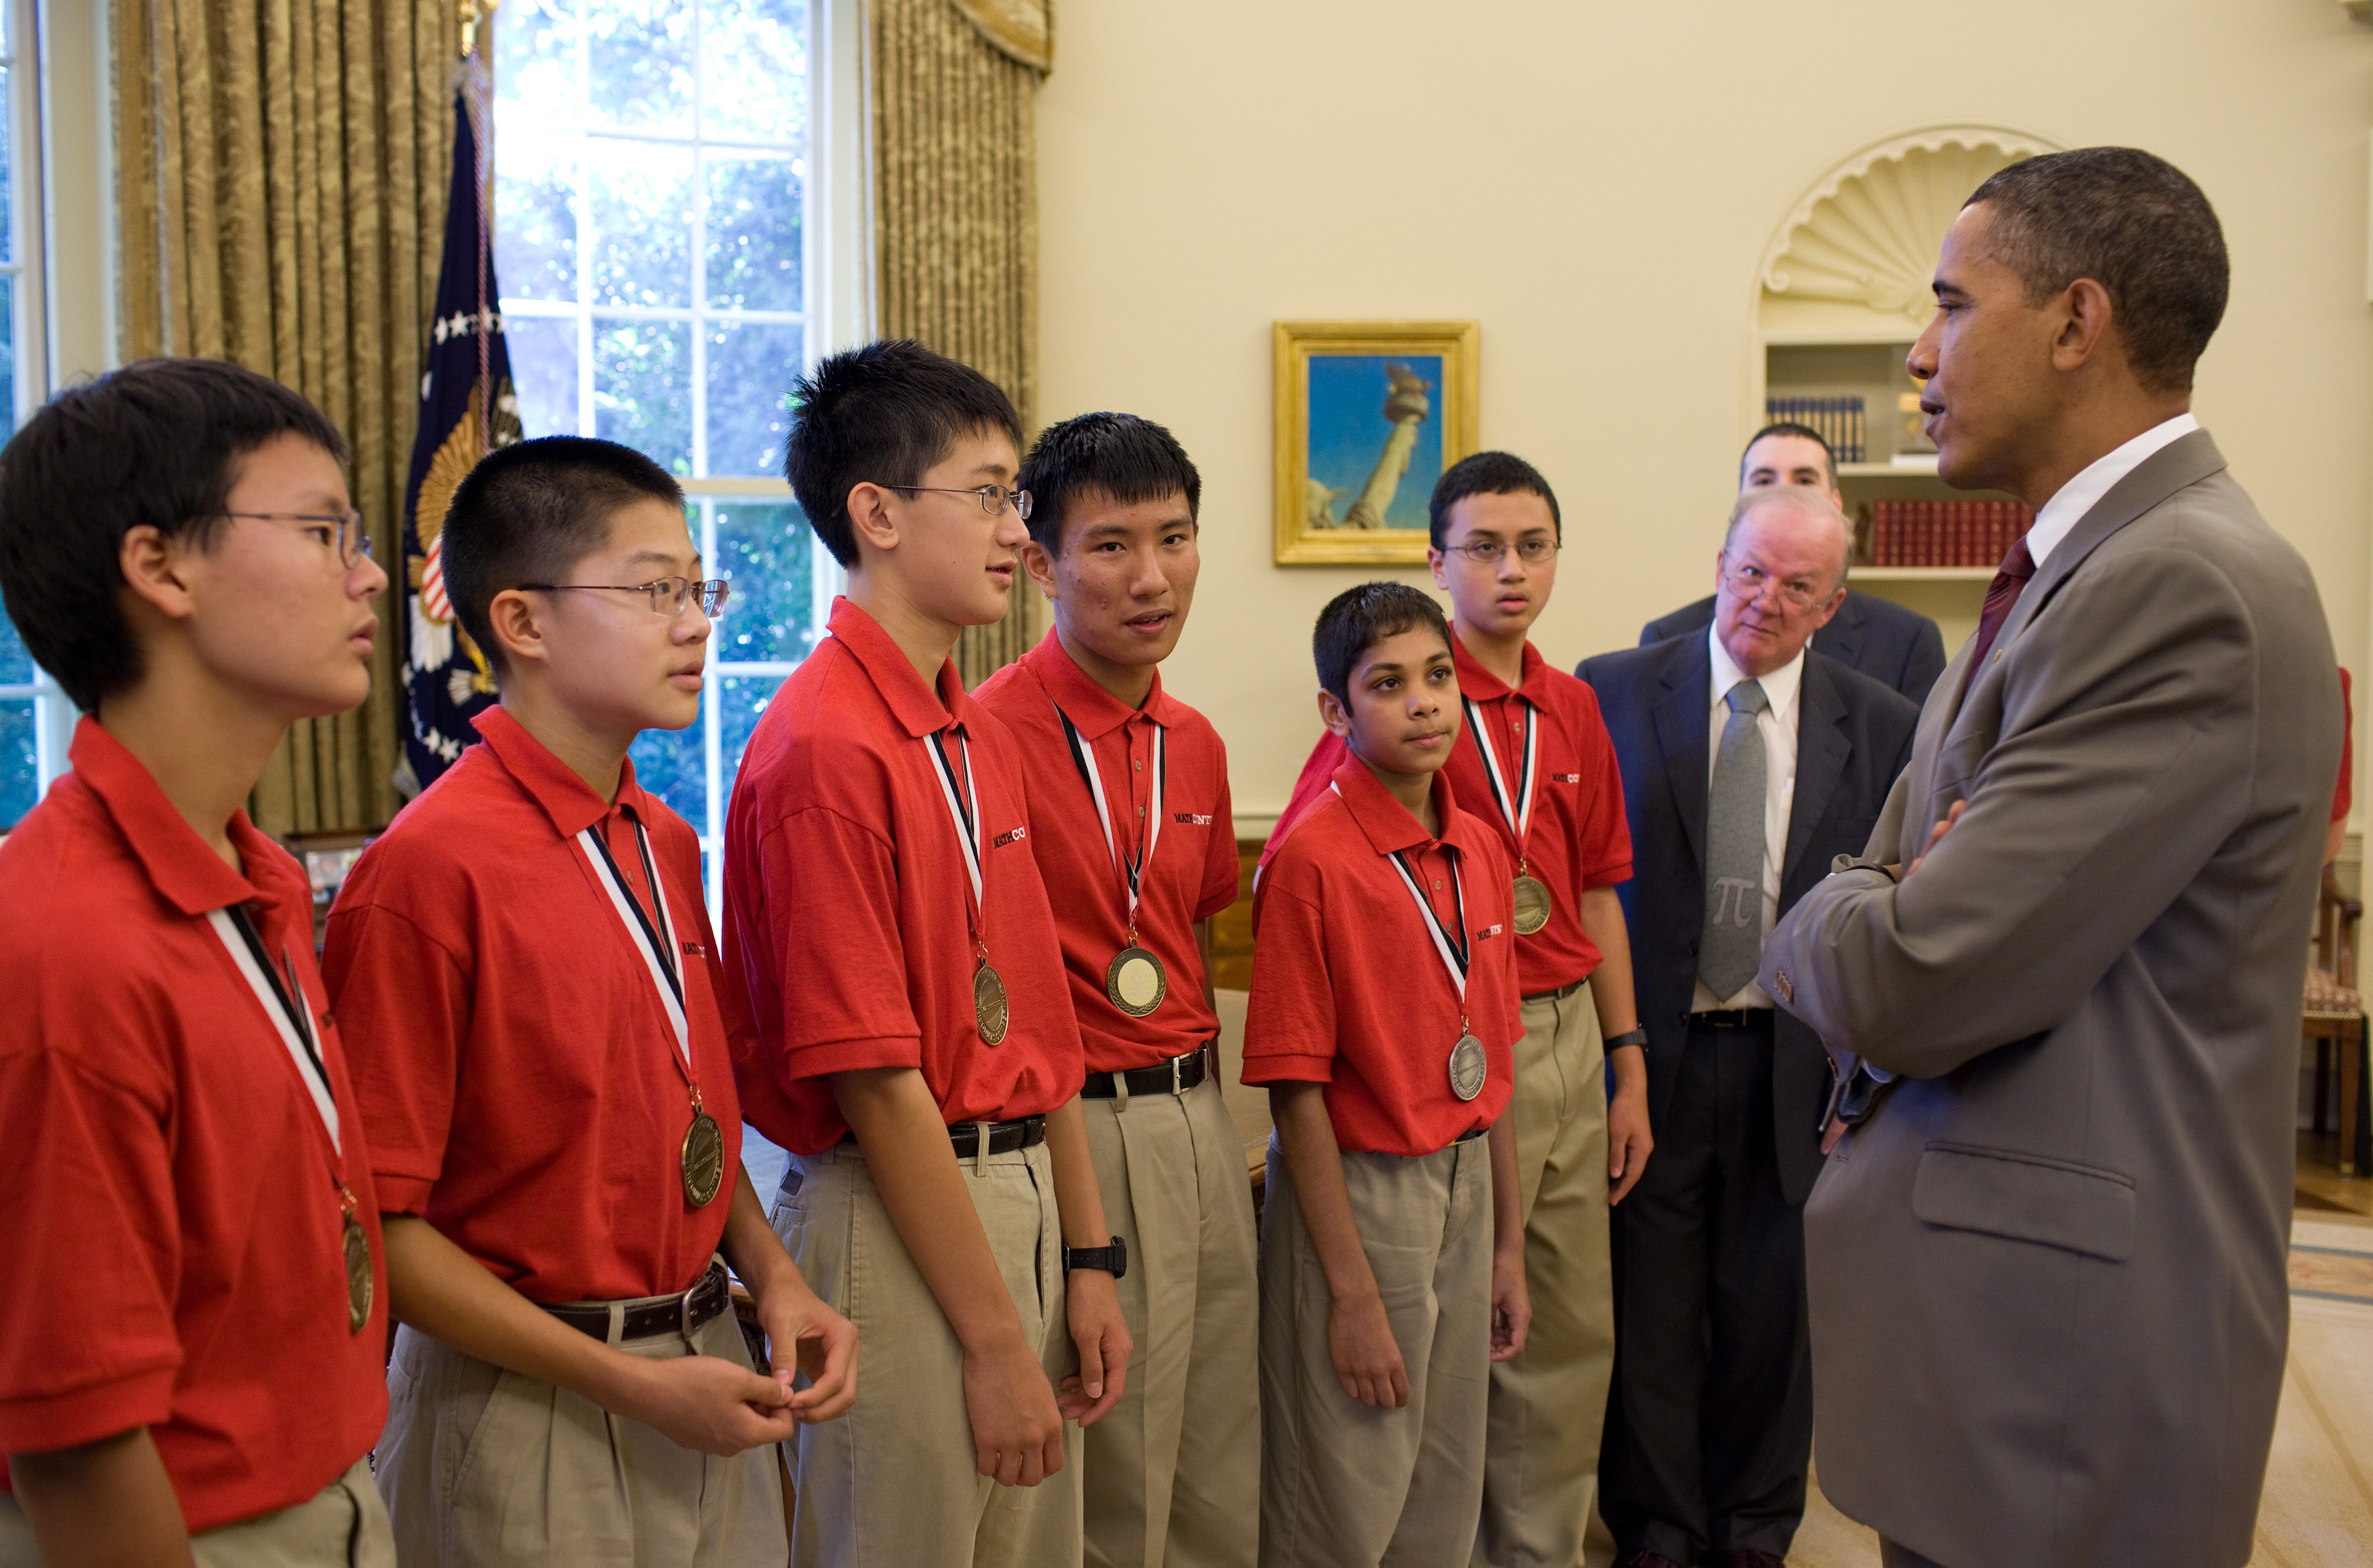
\includegraphics[width=0.6\textwidth]{04 - Number Theory 101/barak.jpg}
      \end{center}
    \end{column}
    \begin{column}{0.5\textwidth}
      The number we just found is called
      \begin{definition}
        The \textbf{Greatest Common Divisor (GCD)} of two counting numbers is the largest counting number that \emph{divides each} of the two given numbers.
      \end{definition}
      
      The GCD of two number is often denoted as $\gcd(a,\ b)$ or simply (in some context) $(a,\ b)$.\medskip

      You've already met the Greatest Common Divisor when study reducing of common fractions.\medskip 

      In the name "greatest common divisor", the adjective "greatest" may be replaced by "highest", and the word "divisor" may be replaced by "factor", so that other names include \textbf{greatest common factor (GCF)}, etc. Historically, other names for the same concept have included the \emph{greatest common measure}.
    \end{column}
  \end{columns}
\end{frame}

\begin{frame}{Finding Greatest Common Divisor}
  \begin{columns}[T]
    \begin{column}{0.5\textwidth}
        To find the \textbf{GCD} of two numbers, it is often helpful to perform a \textbf{prime factorization} of the numbers.

      \begin{definition}
        The GCD is the \textbf{product of all of shared prime factors} of numbers.
      \end{definition}

      \begin{problem}
        What is the GCD of $144$ and $900$?
      \end{problem}
      \vspace*{-1.8ex}
      \[ 144 = 2^4 \cdot 3^2, \qquad 900 = 2^2 \cdot 3^2 \cdot 5^2. \]
      From their prime factorizations, we see that $144$ and $900$ share two factors of $2$ and two factors of~$3$, so $\gcd(144,\ 900) = 2^2 \cdot 3^2 = 36$.

      \begin{example}
        If the GCD of two numbers is $1$, we say the numbers are relatively prime or \textbf{coprime}.                 
      \end{example}
      For example, neither $35$ nor $12$ is a prime number, but they are coprime.\smallskip 

      A prime factorization of huge numbers is a super hard problem. In fact, modern computer security is based that no one can factor huge numbers in a~reasonable time.
    \end{column}
    \begin{column}{0.5\textwidth}
      But sometimes, the prime factorization itself is a~problem. In this case, the \textbf{Euclidean algorithm} will help. It is based on the fact that 
      
      {\centering
      if $a > b$, then $\gcd(a,\ b) = \gcd(a − k \cdot b, b)$.}

      \begin{problem}
        What is the GCD of $833$ and $221$?        
      \end{problem}

      The prime factorization isn’t trivial, so we start with division with a reminder:
      \[ \mathbf{833} = \mathbf{221} × 3 + \mathbf{170}. \]
      So we get, that $\gcd(833, 221) = \gcd(221, 170)$. Then we will do next step and continue until we get a reminder $0$, that means the previous value is the GCD
      \begin{align*}
        \mathbf{221} &= \mathbf{170} × 1 + \mathbf{51}, \\
        \mathbf{170} &= \mathbf{51} × 3 + \mathbf{17}, \\
        \mathbf{51} &= \mathbf{17} × 3 + \mathbf{0}.                 
      \end{align*}
      That reminder $0$ says that $51$ is multiple of $17$, so $\gcd(51,\ 17) = 17$, and that means $\gcd(833,\ 221) = 17$. 
    \end{column}
  \end{columns}
\end{frame}

\begin{frame}{Least common multiple}
  \begin{columns}[T]
    \begin{column}{0.5\textwidth}
      \begin{problem}
        Alice has invited friends to a party and wants to buy cookies for everyone. She knows there will be $24$ or $30$ guests, so she wants that everybody gets an equal amount of cookies. What is the \textbf{minimum} amount of cookies should she buy?
      \end{problem}
      \begin{wrapfigure}[8]{r}{0.34\textwidth}
        \vspace*{-2em}\hspace*{-3em}
        
\includegraphics[width=0.5\textwidth]{04 - Number Theory 101/coockies.png}
      \end{wrapfigure}

      To split~cookies~equally between $24$~friends,~she can buy $24$, $48$,~$72$,~$96$, $120$, $144$, and so on. 

      To~split~cookies~equally between~$30$~friends,~she can buy $30$,~$60$,~$90$,~$120$, $150$, and so on. 
      
      Therefore, we may see, the minimum amount of cookies she should buy is $120$.

      \begin{definition}
        The \textbf{Least Common Multiple (LCM)} of two counting numbers is the smallest counting number that each of the given numbers divides.  
      \end{definition}
    \end{column}
    \begin{column}{0.5\textwidth}
      The LCM of two numbers is often denoted as $\lcm(a,\ b)$ or simply (in some context) $[a,\ b]$. 

      To find the LCM of two numbers performing a \textbf{prime factorization} of the numbers is also helpful. The LCM of two numbers is the product of all primes in \emph{their maximal power} in the factorization of each number.
      
      \begin{definition}
        What is the LCM of $144$ and $900$?        
      \end{definition}
      \vspace*{-1em}
      \[ 144 = 2^4 3^2, \qquad 900 =2^2 3^2 5^2. \]  
      Their prime factorizations show that maximal power of $2$ is $4$, maximal power of $3$ is $2$, and maximal power of $5$ is also $2$. So 
      \[ \lcm(144,\ 900) = 2^4 3^2 5^2 = 3600. \] 
      Curious mind probably noted, that 
      \[ 144 \times 900 = 36 \times 3600 = 129600. \]
      \vspace*{-1\baselineskip}
      \begin{definition}
        Indeed, $a \times b = \gcd(a,\ b) \times \lcm(a,\ b)$, a proof follows from the prime factorization.
      \end{definition}
    \end{column}
  \end{columns}
\end{frame}

\begin{frame}{The Chicken McNuggets Theorem}
  \begin{columns}[T]
    \begin{column}{0.5\textwidth}
      \begin{problem}
        When they were first introduced, McDonald's Chicken McNuggets came in boxes of $9$ or $20$.  What was the largest number of McNuggets that was not expressible as the sum of integer multiples of $9$ and $20$?
      \end{problem}
      {\small
      Let's look at a simpler version of this problem: 
      \begin{problem}
        What is the largest integer that cannot be expressed as the sum of integer multiples of $3$ and $5$?
      \end{problem}

      To find the solution, we need to find the largest integer by counting upwards before we first find \emph{$3$ integers in a row} that can be expressed as the sum of multiples of $3$ and $5$.  After that, we can simply add factors of $3$ to get the series to repeat to infinity.
      \begin{align*}
        6 &= 2 \times 3, \\
        7 &\text{ cannot be expressed}, \\ 
        8 &= 3 + 5, \\
        9 &= 3 \times 3, \\
        10 &= 2 \times 5. 
      \end{align*} 
      So $7$ is the answer.
      }
    \end{column}
    \begin{column}{0.5\textwidth}
      For $9$ and $20$, a lot of counting (or a little computer coding) will tell you the answer is $151$, but we can use the following theorem.
      
      {\color{textBlue} Theorem:}
      \begin{definition}
        For \emph{coprime} integers $m$ and $n$, let $L\{m,\ n\}$ be the largest integer that cannot be expressed as the sum of integer multiples $m$ and $n$. Then
        \[ L\{m,\ n\} = mn − m − n. \]
        \vspace*{-1\baselineskip}
      \end{definition}
      Since $9$ and $20$ are coprime ($\gcd(9,\ 20) = 1$),
      \begin{align*}
        L\{9,\ 20\} &= 9 \times 20 - 9 - 20 = 151, \\
        L\{3,\ 5\} &= 3 \times 5 - 3 - 5 = 7.
      \end{align*}
      \begin{center}
        \vspace*{-1\baselineskip}
        
\includegraphics[width=0.7\textwidth]{04 - Number Theory 101/mcnuggets.png}
      \end{center}
    \end{column}
  \end{columns}
\end{frame}

\begin{frame}{Exercises\hspace*{0.35\textwidth}Challenge Problems}
  \begin{columns}[T]
    \begin{column}{0.5\textwidth}
      \begin{enumerate}
        \item What is the only whole number that is not included in the set of counting numbers?
        \item What is the prime factorization of $144$?
        \item What is the prime factorization of $2021$?
        \item What is the $\gcd(5040,\ 6125)$?
        \item What is the $\lcm(484,\ 330)$?
        \item Larry goes shopping every $3$ days, Moe goes shopping every $4$ days, and Curly goes shopping every $5$ days.  If they all go shopping together on a Sunday, what is the first day of the week they could go shopping together again?
        \item In a video game, red aliens are worth $7$ points and blue aliens are worth $9$ points.  What is the highest score that can’t be obtained by capturing only red or blue aliens.
        \item What is the product when the $\lcm (a,\ b)$ is multiplied by the $\gcd (a,\ b)$?
      \end{enumerate}
    \end{column}
    \begin{column}{0.5\textwidth}
      \begin{enumerate}
        \item What is the largest integer that can’t be expressed as the sum of integer multiples of $5$, $7$, $8$?

        \item Find the smallest positive integer which\\ when divided by $12$ leaves a remainder of $11$, when divided by $11$ leaves a remainder of $10$, when divided by $10$ leaves a remainder of $9$, etc. down to where, when divided by $2$, it leaves a remainder of $1$.

        \item Find the smallest positive integer greater than $1$ which yields a remainder of $1$ when divided by any single digit positive integer greater than $1$.
      \end{enumerate}
    \end{column}
  \end{columns}
\end{frame}

% \begin{frame}{Title}
%   \begin{columns}[T]
%     \begin{column}{0.5\textwidth}
%     \end{column}
%     \begin{column}{0.5\textwidth}
%     \end{column}
%   \end{columns}
% \end{frame}

\end{document}
